\vspace*{\subsecspace}
%\section{Experimental Evaluation}
%\section{Model Testing and Validation}
\section{Testing and Evaluation of Model-Informed Policies}
\label{sec:eval}

%\vspace*{\subsecspace}
%\section{SciSpot Design and Implementation}
\subsection{Details of the Experimental Framework used for Evaluation}
%\section{Model-Informed Policy Implementation}
\label{sec:impl}


\sysname is a general-purpose software framework for running scientific computing applications on low-cost transient cloud servers.
It incorporates policies and mechanisms for generating, deploying, orchestrating, and monitoring bags of jobs on cloud servers.
Specifically, it runs a bag of jobs defined by these parameters:
\begin{lstlisting}[basicstyle=\sffamily, frame=single, columns=fullflexible, escapeinside={(*}{*)}]
  Bag of job = {(*$\mathcal{A}$*): Application to execute,
  (*$n$*): Number of jobs,
  (*$m$*): Minimum number of jobs to finish,
  (*$\pi$*): Generator function for job parameters,
  (*$\mathcal{R}$*): Computing resources per job}
\end{lstlisting}


%Additionally, ease-of-use is one of \sysname's primary design goals, and we specifically incorporate

%it is suitable for running a large variety of applications.
\sysname seeks to minimize the cost and running time of bags of jobs of scientific computing applications.
\sysname's cost and time minimizing policies for running bags of jobs are based on empirical and analytical models of the cost and preemption dynamics of  transient cloud servers, which we present in the next section. 

\sysname is designed as a framework that increases the usability and viability of transient cloud servers for scientific computing applications, and provides a simple user interface to allow users to deploy their applications with minimum workflow changes. 
Most scientific computing applications are deployed on HPC clusters that have a batch scheduler such as Slurm~\cite{slurm} or Torque~\cite{torque}, and \sysname integrates with these schedulers (e.g., Slurm) to provide the same interface to applications. 
As shown in Figure~\ref{fig:arch},
\sysname creates and manages clusters of transient cloud servers, manages all aspects of the VM lifecycle and costs, and implements the various policies described in the rest of this section. 

\begin{figure}[t]
  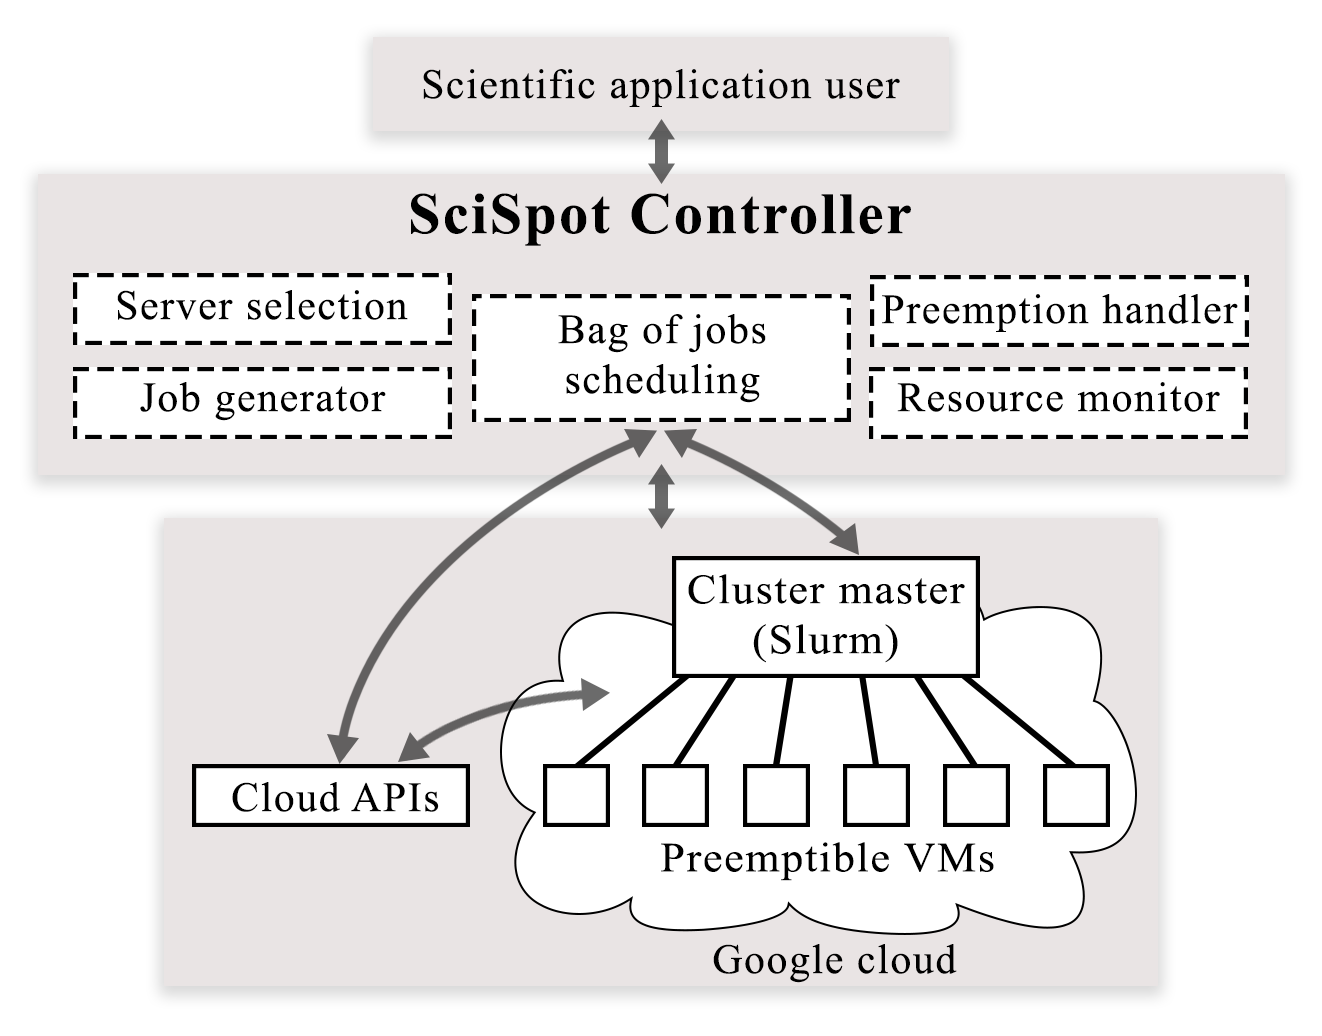
\includegraphics[width=0.3\textwidth]{../figures/Architecture.png}
\vspace*{\myfigspace}
  \caption{SciSpot architecture and system components.}
  \label{fig:arch}
  \vspace*{\myfigspace}
\end{figure}


\noindent \textbf{High-level workflow:} When a user wishes to run a bag of jobs, \sysname handles the provisioning of a cluster of transient cloud servers.
In addition, \sysname deals with the scheduling and monitoring of the bag of jobs, and with VM preemptions. 
Execution of a bag of jobs proceeds in two phases.
In the first phase, \sysname selects the ``right'' cluster configuration for a given application through a cost-minimizing exploration-based search policy, described in Section~\ref{subsec:server-selection}. 
In the second phase, \sysname proceeds to run the remaining jobs in the bag on the optimal cluster configuration. 

\prat{End design}


\sysname is implemented as a light-weight, extensible framework that makes it convenient and cheap to run scientific computing applications in the cloud.
We have implemented the \sysname prototype in Python in about 2,000 lines of code, and currently support running VMs on the Google Cloud Platform~\cite{gcp}. 
%
\sysname is implemented as a centralized controller, which implements the VM selection and job scheduling policies described in Section~\ref{sec:design}. 
The controller can run on any machine (including the user's local machine, or inside a cloud VM), and exposes an HTTP API to end-users. 
Users submit bags of jobs to the controller via the HTTP API, which then launches and maintains a cluster of cloud VMs, and maintains the job queue and metadata in a local database. 
To improve usability, we automatically generate parameter combinations for a given bag size, based on a user-provided json file with ranges and constraints for each parameter. 

\sysname integrates, and interfaces with two primary services.
First, it uses the Google cloud API~\cite{gcloud-api} for launching, terminating, and monitoring VMs.
Once a cluster is launched, it then configures a cluster manager such as Slurm~\cite{slurm} or Torque~\cite{torque}, to which it submits jobs. 
\sysname uses the Slurm cluster manager, with each VM acting as a Slurm ``cloud'' node, which allows Slurm to gracefully handle VM preemptions.
The Slurm master node runs on a small, 2 CPU non-preemptible VM, which is shared by all applications and users. 
\sysname monitors job completions and failures (due to VM preemptions) through the use of Slurm call-backs, which issue HTTP requests back to the \sysname controller.

%As part of \sysname, we also provide a base VM image with Slurm and MPI integration, along with commonly used libraries and benchmarks for scientific computing. To run an application, users must provide a location to the application source code or binaries. Integrating \sysname with container-based image management tools such as Docker~\cite{docker} and Singularity~\cite{kurtzer2017singularity} is part of our ongoing work. 





%%% Local Variables:
%%% mode: latex
%%% TeX-master: "paper"
%%% End:


%Opening is deliberately short because we gonna be running out of space 
In this section, we present empirical and analytical evaluation of the performance and cost of \sysname with different scientific computing workloads and scales. 
Our evaluation consists of empirical analysis, as well as model-driven simulations for analyzing and comparing \sysname behavior under different preemption and application dynamics.

We shed insight into the fundamental tradeoffs in constrained preemptions, the effectiveness of our model-based policies, and detailed empirical analysis of the cost and performance of our \sysname framework with real-world scientific computing applications. 
We have already established the goodness of fit of our model and compared it to existing models earlier in Section~\ref{sec:failmodel}. 

% \begin{itemize}
% \item What is performance and cost of 
% \end{itemize}

\noindent \textbf{Environment and Workloads:} All our empirical evaluation is conducted on the Google Public Cloud, and with these representative scientific computing applications: 
% open-source
%\vspace*{\tightext}
%\begin{description}
  %TODO: Need MAX two sentence descriptions

\noindent \textbf{Nanoconfinement.}
The nanoconfinement application launches molecular dynamics (MD) simulations of ions in nanoscale confinement created by material surfaces \cite{jyto,kadupitiya2017}.

\noindent \textbf{Shapes.} The Shapes application runs an MD-based optimization dynamics to predict the optimal shape of deformable, charged nanoparticles \cite{jto1,jjzo1}. 

\noindent \textbf{LULESH.} Livermore Unstructured Lagrangian Explicit Shock Hydrodynamics (LULESH)  is a popular benchmark for hydrodynamics simulations of continuum material models \cite{IPDPS13:LULESH,LULESH2:changes}. 
% \end{description}

These examples are representative of typical scientific computing applications in the broad domain of physics, materials science, and chemical engineering. These three examples are implemented as parallel programs that use OpenMP and MPI parallel computing techniques. The first two are used in nanoscale materials research \cite{jso1,jso2,solis2013generating,jjzo1,jto1,jyto} and LULESH is a widely used benchmark \cite{IPDPS13:LULESH,LULESH2:changes}.
All applications are run with default parameters unless otherwise stated. 


All applications use OpenMPI v2.1.1, are deployed on Slurm v0.4.3 and 64-bit Ubuntu 18.04, and run on Google Cloud VMs with x86-64 Intel Haswell CPUs. 
% Networking?
For completeness and to guard against concerns about poor cloud performance relative to HPC clusters ~\cite{iosup_performance_2011, zhai_cloud_2011, marathe2013comparative, galante_analysis_2016, benedictis_cloud-aware_2014}, we benchmarked the Nanoconfinement application on the Big Red II cluster~\cite{bigred2}. 
When run on 4 nodes with 16 CPUs each, the application takes 1140 seconds on Big Red II vs 850 seconds on \sysname. 
We attribute the 20\% improvement with \sysname to the newer CPUs on Google Cloud (Intel Haswell vs. older 2012-era AMD Opterons in Big Red II).

%For completeness, we show the running times on the Big Red II supercomputing cluster in Table~\ref{tab:bigred2}, with 16 CPU nodes used throughout, and we see that our representative applications \emph{do not} face a penalty when deployed on the cloud. 

\vspace*{\subsecspace}

\subsection{Tradeoffs In Constrained Preemptions}

Below, we analyze the effect of the bathtub shaped preemption curve on application running time. 


Preemptions cause jobs to be restarted, which is the \emph{wasted} time, which increases the total running time (i.e, makespan).
In the case of constrained preemptions, we evaluate two preemption probability, the empirically observed bathtub shaped and a uniform distribution of failures.


In Figure~\ref{fig:vs-uniform} we show the expected wasted time \emph{assuming the job suffers a single failure.}
We see that in the case of uniform distribution, the increase is linear in the job length.
Whereas with bathtub shaped distributions, the mirrors the shape of the CDF, and is constant for all but the largest of jobs. 


The expected wasted time is also influenced by the probability of failure, and Figure~\ref{fig:vs-uniform-2} shows the expected waste.
Because preemption rate is high in the initial stages for bathtub failures, for short jobs, the expected waste is higher, because they do not run long enough to take advantage of the low rate of preemptions in the middle stages.
If preemptions were uniformly distributed, the waste is \emph{quadratic}, and given by $\frac{T^2}{48}$, and is smaller for short jobs. 
We see that the ``cross over'' point is around 5 hours---and for longer jobs, a bathtub preemption behavior is preferable.

\prat{Do we give the equations here, or earlier?}


\begin{figure}
  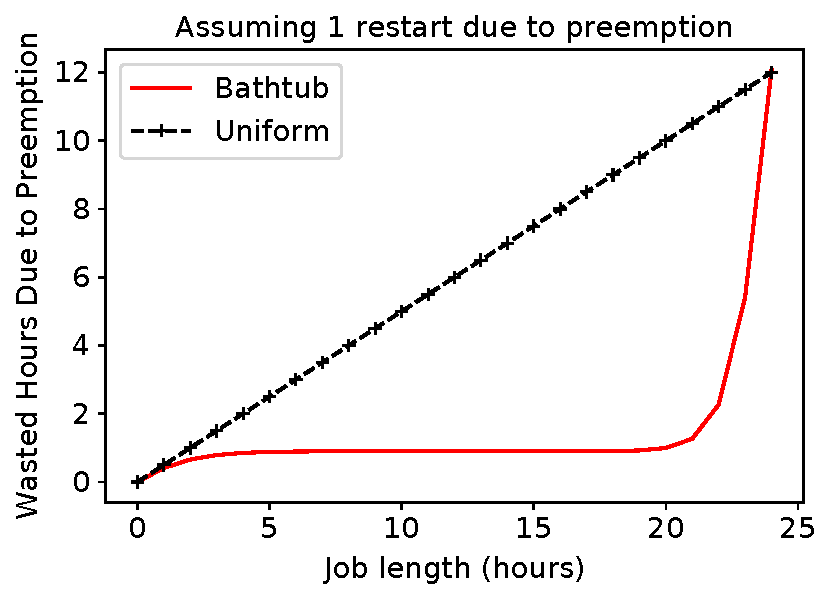
\includegraphics[width=0.4\textwidth]{../graphs/uniform-v-bathtub.pdf}
  \caption{The expected wasted computation, given a single failure, is lower when preemptions are distributed in a bathtub shape, compared to uniformly distributed over the 24 hour interval}
  \label{fig:vs-uniform}
\end{figure}

\begin{figure}
  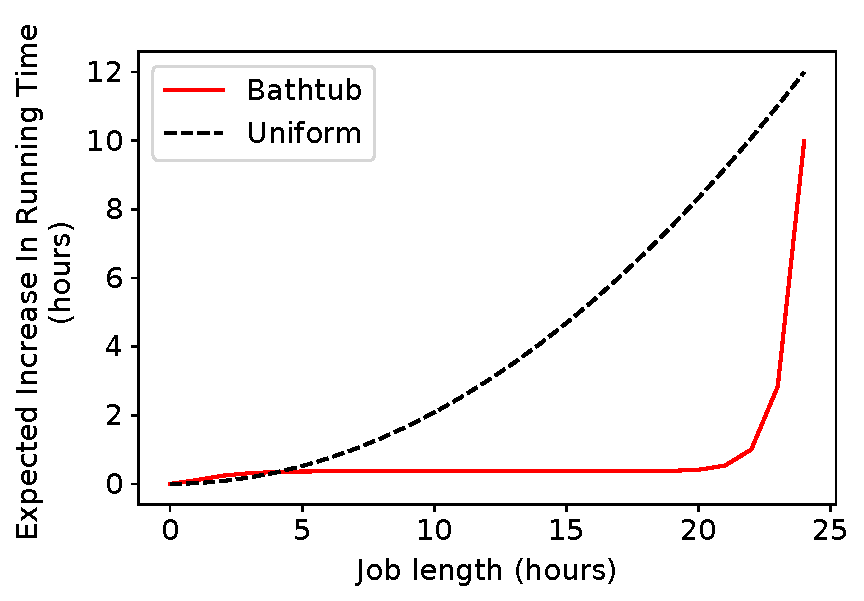
\includegraphics[width=0.4\textwidth]{../graphs/uniform-v-bathtub-2.pdf}
  \caption{The expected wasted computation is lower when preemptions are distributed in a bathtub shape, compared to uniformly distributed over the 24 hour interval}
  \label{fig:vs-uniform-2}
\end{figure}

\noindent \textbf{Result:} \emph{For constrained preemptions, bathtub distributions significantly reduce the expected increase in running times for medium to long running jobs, but are slightly inferior for short jobs.}

%%%%%%%%%%%%%%%%%%%%%%%%%%%%%%%%%%%%%%%%%%%%%%%%%%%%%%%%%%%%%%%%%%%%%%
\subsection{Model-based Policies}
\label{subsec:eval-policy}

We now evaluate our model-driven policies. 


\subsubsection{Scheduling}

Our job scheduling policy is model-driven and decides whether to request a new VM for a job or run on an existing VM.

Figure~\ref{fig:sched-bathtub} shows the effect of this policy for a job of length 4 hours.
We compare against a baseline of existing scheduling policies used by other systems such as ExoSphere .
In the absence of insights about bathtub preemptions, the existing frameworks would continue to run on existing server.
As the figure shows, for larger jobs the job failure probability is high. 

\begin{figure}[t]
  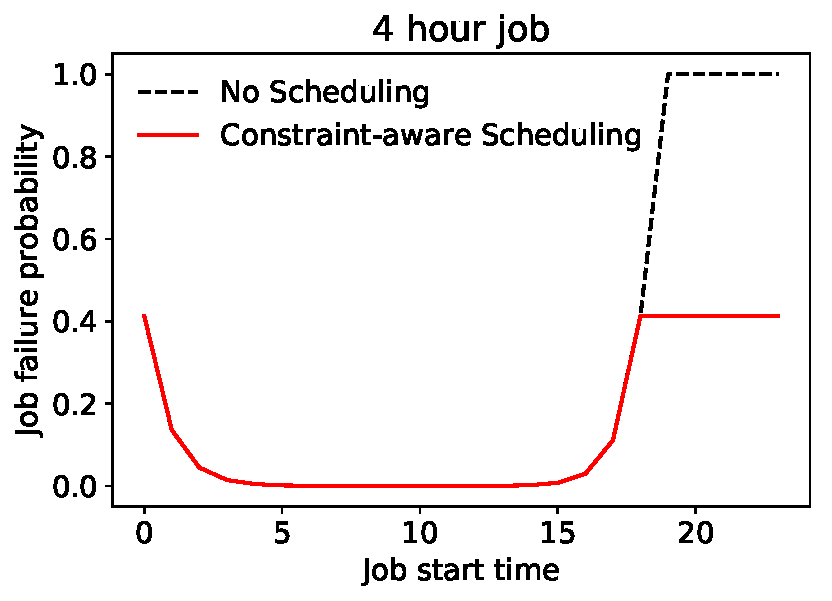
\includegraphics[width=0.4\textwidth]{../graphs/Sched-bathtub.pdf}
  \caption{Job failure probability is reduced with the help of our deadline aware scheduling policy, especially for jobs starting near the end of the VM's lifetime}
  \label{fig:sched-bathtub}
\end{figure}


Figure~\ref{fig:sched-all} shows the job failure probability for jobs of differen sizes for our model based policy vs a existing vanilla ``null'' policies that are not informed by the preemption dynamics.



\begin{figure}[t]
  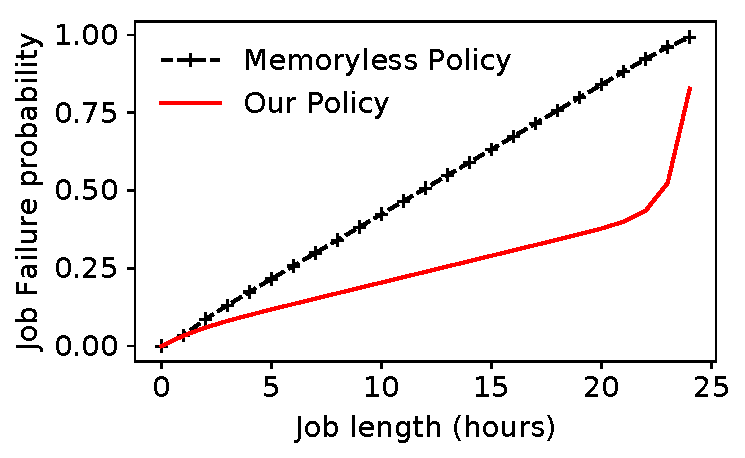
\includegraphics[width=0.4\textwidth]{../graphs/Sched-fail-prob.pdf}
  \caption{Job failure probability is lower with our deadline aware policy across all job sizes}
  \label{fig:sched-all}
\end{figure}



%%%%%%%%%%%%%%%%%%%%%%%%%%%%%%%%%%%%%%%%%%%%%%%%%%
\subsubsection{Checkpointing}
\label{subsec:eval-ckpt}


\begin{figure}[t]
  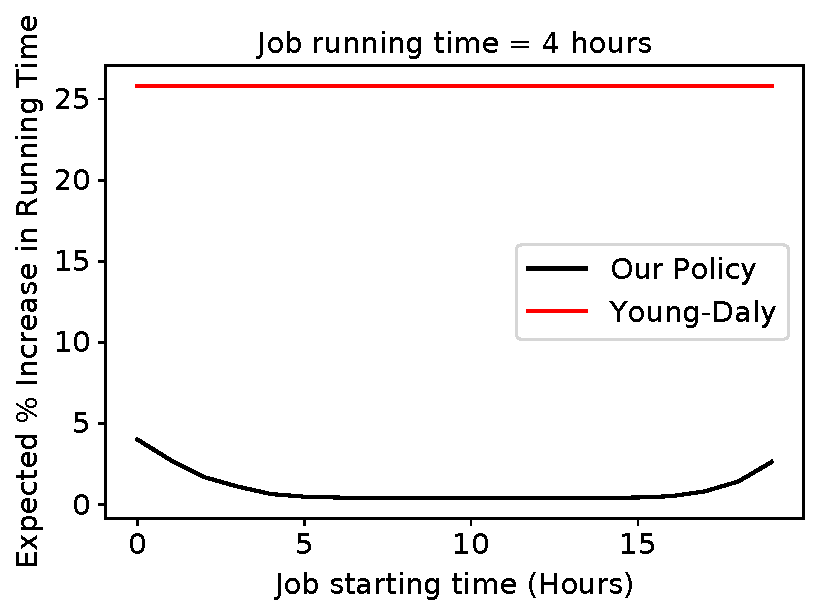
\includegraphics[width=0.4\textwidth]{../graphs/ckpt-4.pdf}
  \caption{Checkpointing overhead for jobs of length 4 at different starting times.}
  \label{fig:ckpt-4}
\end{figure}

\begin{figure}
  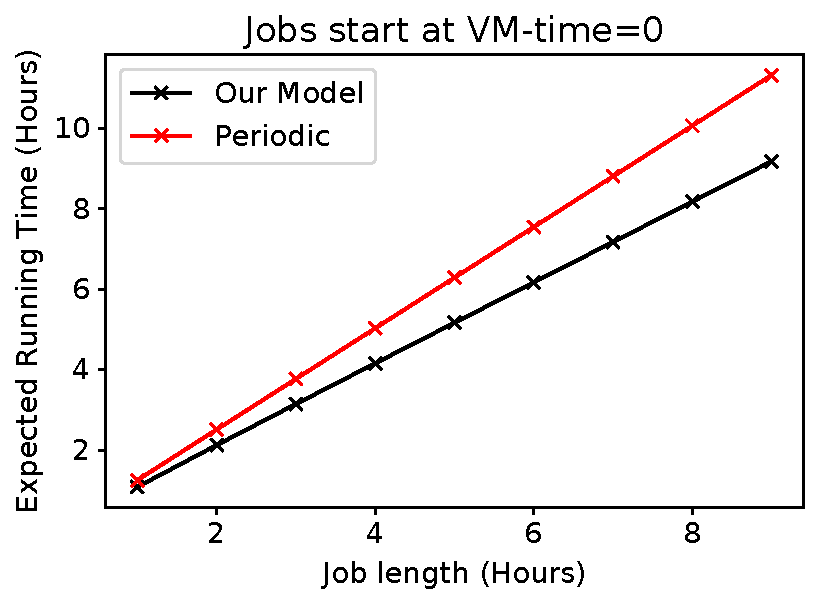
\includegraphics[width=0.4\textwidth]{../graphs/ckpt-start-0.pdf}
  \caption{Running time with checkpointing when jobs start at time=0}
  \label{fig:ckpt-start-0}
\end{figure}


\begin{figure}
  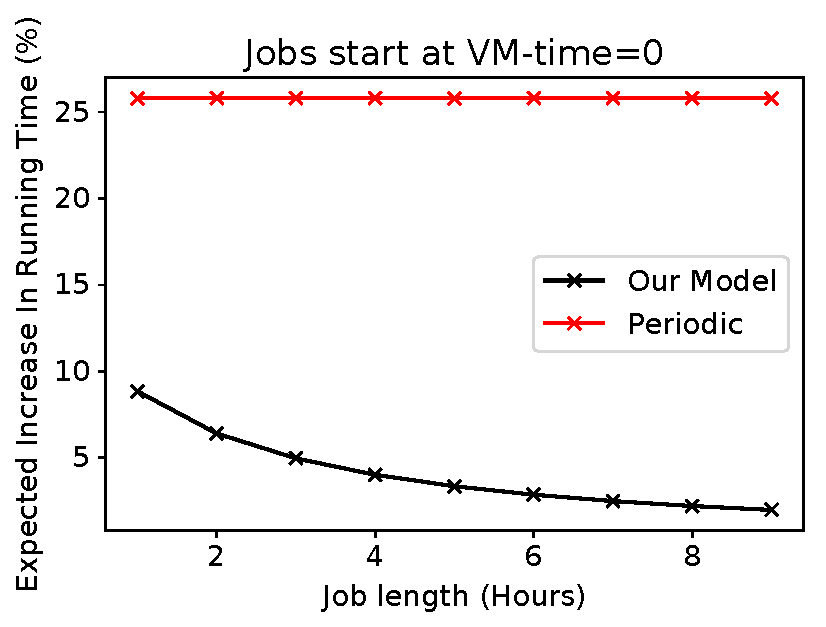
\includegraphics[width=0.4\textwidth]{../graphs/ckpt-start-relative.pdf}
  \caption{Increase in running time with Checkpointing when jobs start at time =0 (Should be an inset}.
  \label{fig:ckpt-start-0-relative}
\end{figure}


%%%%%%%%%%%%%%%%%%%%%%%%%%%%%%%%%%%%%%%%%%%%%%%%%%

\begin{comment}
\subsubsection{Server Selection}
\label{subsec:eval-serversel}

When an application (i.e., bag of jobs) requests a total number of CPUs to run each of its jobs, \sysname first runs its exploration phase to find the ``right'' VM for the application.
\sysname searches for the VM that minimizes the total expected cost $E[C_{(i,n_i)}]$ of running the application. %and this depends on several factors such as the parallel structure of the application, the preemption probability and the associated job recomputation time, and the price of the VM.
Thus, even if the \emph{total} amount of resources (i.e., number of CPUs) per job is held constant, the total running time (i.e., turnaround time) of an application depends on the choice of the VM type ($i$), and the associated number of VMs ($n_i$) required to meet the allocation constraint (Section~\ref{subsec:cost-model}).
%
With preemptible instances, the total running time of a job is composed of two factors: the ``base'' running time of the job without any preemptions ($T_{(i,n_i)}$), and the expected recomputation time which depends on the probability of job failure (Equation~\ref{eq:recomput}). 

\begin{figure}
  \centering
  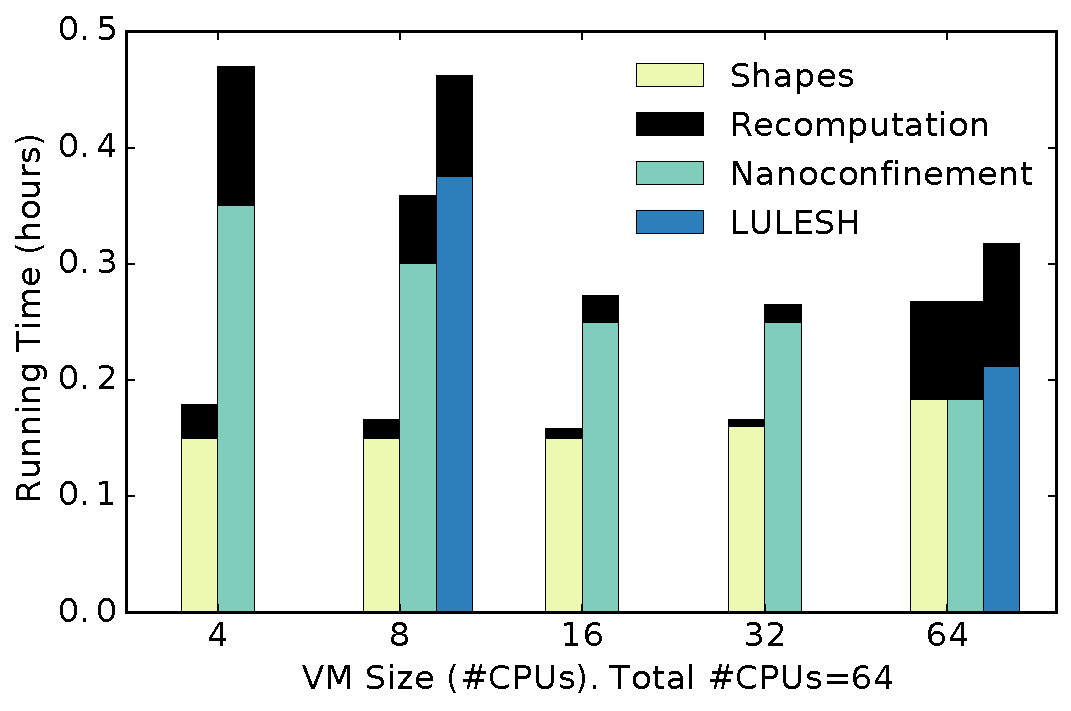
\includegraphics[width=0.4\textwidth]{../graphs/runtime-bars.pdf}
      \vspace*{\myfigspace}
  \caption{Running times of applications on different VMs. Total number of CPUs is 64, yielding different number of VMs in each case. We see different tradeoffs in the base running times and recomputation times.}
  \label{fig:runtimes-bar}
    \vspace*{\myfigspace}
\end{figure}


Figure~\ref{fig:runtimes-bar} shows the running times of the Nanoconfinement, Shapes, and LULESH applications, when they are deployed on different VM sizes. 
In all cases, the total number of CPUs per job is set to 64, and thus the different VM sizes yield different cluster sizes (e.g., 16 VMs with 4 CPUs or 32 VMs with 2 CPUs).
LULESH requires CPUs to be cube of an integer, which limits the valid cluster configurations. 

For Nanoconfinement and LULESH, we observe that the base running times (without preemptions) reduce when moving to larger VMs, because this entails lower communication costs.
For Nanoconfinement, the running time on the ``best'' VM (i.e., with 32 CPUs) is nearly 40\% lower as compared to the worst case. 
On the other hand, the Shapes application can scale to a larger number of VMs without any significant communication overheads, and does not see any significant change in its running time. 

Figure~\ref{fig:runtimes-bar} also shows the expected turnaround time $E[\mathcal{T}_{(i,n_i)}]$, that is obtained by adding the the expected recomputation time, which depends on the expected lifetimes of the VM and the number of VMs, and is computed using the cost model introduced in Section~\ref{subsec:cost-model}. 
While selecting larger VMs may reduce communication overheads and thus improve performance, it is not an adequate policy in the case of preemptible VMs, since the preemptions can significantly increase the turnaround time.
Therefore, even though the base running time of Nanoconfinement is lower on a 64 CPU VM, the recomputation time on the 64 CPU VM is almost $4\times$ higher compared to a 2x32-CPU cluster,  due to the much lower expected lifetime of the larger VMs. 
Thus, on preemptible servers, there is a tradeoff between the base running time which only considers parallelization overheads, and the recomputation time.
By considering \emph{both} these factors, \sysname's server selection policy can select the best VM for an application. 

\prat{Show Scispot selection and naive selection in the graph}

\noindent \emph{\textbf{Result:} Our server selection policy, by considering both the base running time and recomputation time, can improve performance by up to 40\% , and can keep the increase in running time due to recomputation to less than 5\%.}

\end{comment}

%\subsection{SciSpot Evaluation}
\subsection{Evaluation using Typical User-End Scientific Computing Applications}

We show the empirical cost and performance and effectiveness of our \sysname framework which incorporates our model-based insights and is an easy to use integrated Framework for scientific computing applications. 


%%%%%%%%%%%%%%%%%%%%%%%%%%%%%%%%%%%%%%%%%%%%%%%%%%
\subsubsection{Cost}

%As described in Section~\ref{sec:design}, applications can be deployed on multiple types of VMs in the cloud, with each VM type having a different ``size''.
%In our evaluation of parallel scientific computing applications that are CPU intensive, we are primarily interested in the number of CPUs in a VM.


%%%%%%%%%%%%%%%%%%%%%%%%%%%%%%%%%%%%%%%%%%%%%%%%%%


\begin{figure}
  \centering
  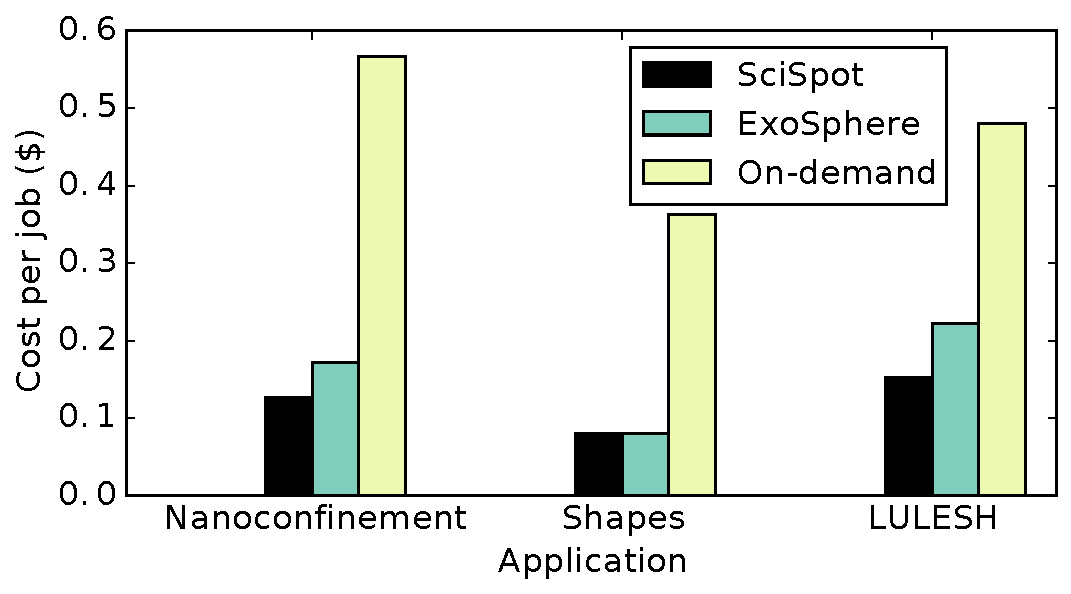
\includegraphics[width=0.4\textwidth]{../graphs/cost-vs-exosphere.pdf}
  \vspace*{\myfigspace}
  \caption{SciSpot's use of preemptible VMs can reduce costs by up to $5\times$ compared to conventional cloud deployments, and 20\% compared to the state of the art EC2 spot instance selection (ExoSphere~\cite{exosphere}).}
  \label{fig:cost-only-bar}
    \vspace*{\myfigspace}
\end{figure}

The primary motivation for using preemptible VMs is their significantly lower cost compared to conventional ``on-demand'' cloud VMs that are non-preemptible. 
Figure~\ref{fig:cost-only-bar} compares the cost of running different applications with different cloud VM deployments. 
\sysname, which uses both cost-minimizing server selection, and preemptible VMs, results in significantly lower costs across the board, even when accounting for preemptions and recomputations. 
%
We also compare against ExoSphere~\cite{exosphere}, a state of the art  system for transient server selection.
ExoSphere implements a portfolio-theory approach using EC2 spot prices to balance average cost saving and risk of revocations using diversification and selecting VMs with low price correlation.
However, this approach is ineffective for the flat prices of Google Preemptible VMs. 
Unlike \sysname, ExoSphere does \emph{not} consider application performance when selecting servers, and thus is unable to select the best server for parallel applications. 
Since the Google \texttt{highcpu} VMs have the same price per CPU, ExoSphere picks an arbitrary ``median'' VM to break ties, which may not necessarily yield the lowest running times.
This results in 20\% cost increase over \sysname. 

\noindent \emph{\textbf{Result:} SciSpot reduces computing costs by up to 5$\times$ compared to conventional on-demand cloud deployments.}




%%%%%%%%%%%%%%%%%%%%%%%%%%%%%%%%%%%%%%%%%%%%%%%%%%
%HPC should be the last thing ?


% \begin{figure}
%   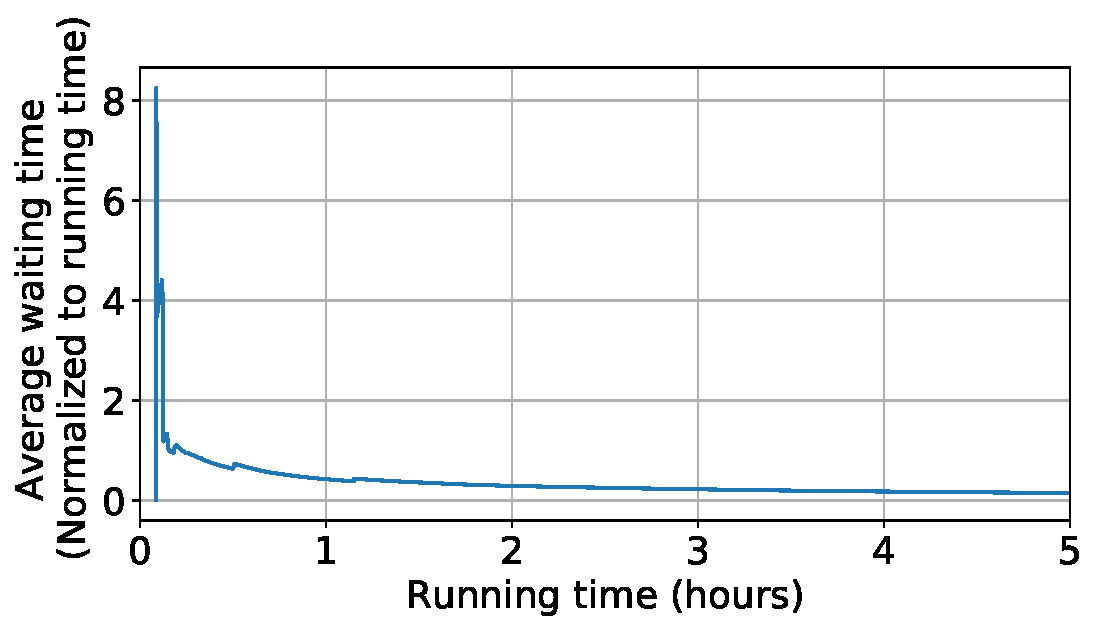
\includegraphics[width=0.4\textwidth]{../data/waiting_cumul.pdf}
%   \caption{The average waiting time (normalized to running time) of jobs of different length.}
%   \label{fig:hpc-wait-cdf}
% \end{figure}



%%% Local Variables:
%%% mode: latex
%%% TeX-master: "paper"
%%% End:
